Contrast enhancement may be described as the process of optimizing the quality of the image in human visual criteria. Histogram equalization is one of the techniques to perform contrast enhancement and works in an image by mapping the distribution of its gray levels to an approximately uniform distribution. The performance of this process is deeply related to the amount of noise in the image since it consists of peaks in the histogram, which unbalances the mapping and enhances noisy structures. One solution to this problem, according to \citeonline{zuiderveld1994constrast}, is to divide the image into \emph{contextual regions}, i.e. rectangular areas of $8 \times 8$ size, compute the optimal contrast for each of the regions and merge the results with bilinear interpolation to avoid boundary effects. This method is known as \sigla{AHE}{Adaptive Histogram Equalization}, where the global outlier gray levels do not influence each contextual region contrast enhancement.

The \sigla{CLAHE}{Contrast Limited Adaptive Histogram Equalization} method was proposed to overcome the drawback of noise. As stated by \citeonline{sonali2019approach}, it is the method that improves the low contrast issue and operates by limiting the contrast enhancement that is usually performed by ordinary histogram equalization or the AHE, which results in the noise enhancement as well. It is accomplished by allowing only a maximum number of pixels in each of the histogram bins and equally distributing the clipped pixels among the whole histogram \cite{zuiderveld1994constrast}. \autoref{fig:hr_ahe_clahe} presents an example of the differences between histogram equalization techniques and their results in a \sigla{MRI}{Magnetic Resonance Imaging} example:

\begin{figure}[htb]
	\caption{\label{fig:hr_ahe_clahe} MRI image of a human knee \textbf{(a)}, a simple histogram equalization \textbf{(b)}, an adaptive histogram equalization \textbf{(c)} and the contrast limited adaptive histogram equalization \textbf{(d)}.} 
	\begin{center}
	    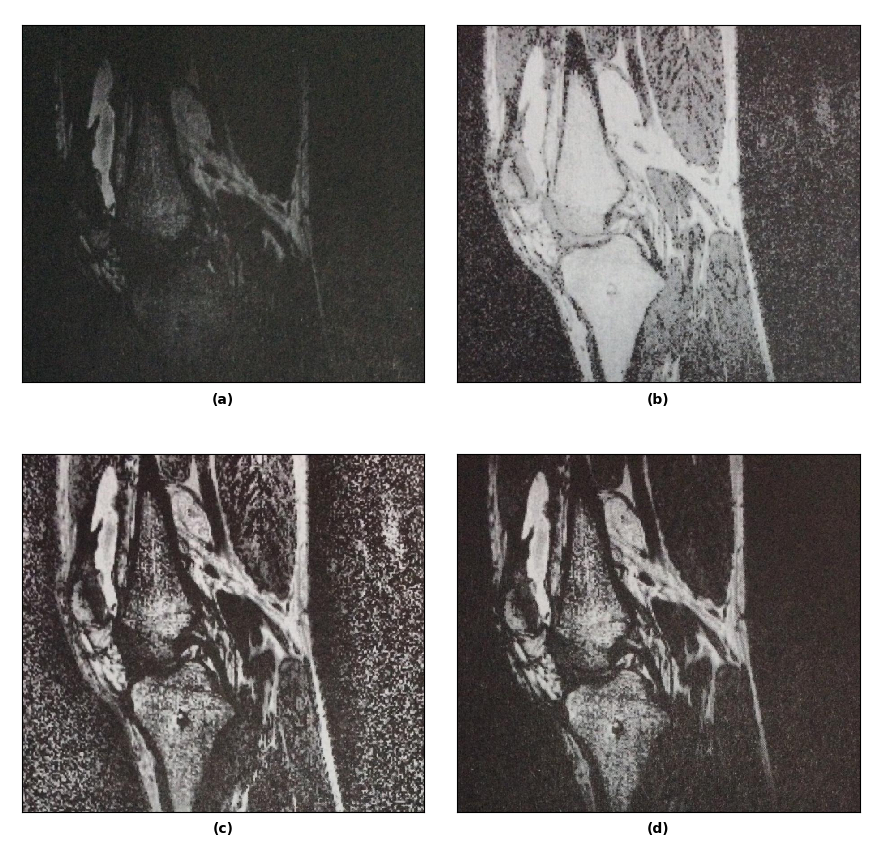
\includegraphics[scale=0.4]{images/knee_HE_AHE_CLAHE.png}
	\end{center}
	\centering
    \fadaptada{zuiderveld1994constrast}
\end{figure}
